% Created 2024-07-26 Fri 14:27
% Intended LaTeX compiler: pdflatex
\documentclass[letterpaper, 12pt]{article}
\usepackage[utf8]{inputenc}
\usepackage[T1]{fontenc}
\usepackage{graphicx}
\usepackage{longtable}
\usepackage{wrapfig}
\usepackage{rotating}
\usepackage[normalem]{ulem}
\usepackage{amsmath}
\usepackage{amssymb}
\usepackage{capt-of}
\usepackage{hyperref}
\usepackage{minted}
\usepackage{xcolor}
\usepackage{hyperref}
\usepackage{tocloft}
\usepackage{minted}
\usemintedstyle{manni}
\usepackage{pdfpages}
\usepackage{fancyhdr}
\usepackage{graphicx}
\usepackage[top=1.4in, left=0.5in, right=0.5in, bottom=0.8in]{geometry}
\usepackage[T1]{fontenc}
\usepackage{helvet}
\pagestyle{fancy}
\renewcommand{\headrulewidth}{0pt}
\renewcommand{\footrulewidth}{0pt}
\setlength{\parindent}{0em}
\setlength{\parskip}{1em}
\usepackage{hyperref}
\usepackage{color}
\hypersetup{
colorlinks=true,
linkcolor=blue,
filecolor=magenta,
urlcolor=cyan,
citecolor=green,
pdfborder={0 0 0}
}
\addtolength{\evensidemargin}{-2in}
\addtolength{\topmargin}{-0.5in}
\addtolength{\textwidth}{0in}
\usepackage[most]{tcolorbox}
\author{Hilduara Abreu}
\date{\today}
\title{Carta de Bienvenida K-5\\\medskip
\large llegadanuevo ano escolar 2024-25}
\hypersetup{
 pdfauthor={Hilduara Abreu},
 pdftitle={Carta de Bienvenida K-5},
 pdfkeywords={},
 pdfsubject={},
 pdfcreator={Emacs 29.4 (Org mode 9.6.15)}, 
 pdflang={English}}
\begin{document}

\fancyfoot[C]{\setlength{\unitlength}{1in}\begin{picture}(5,0)\put(-1.8,-1){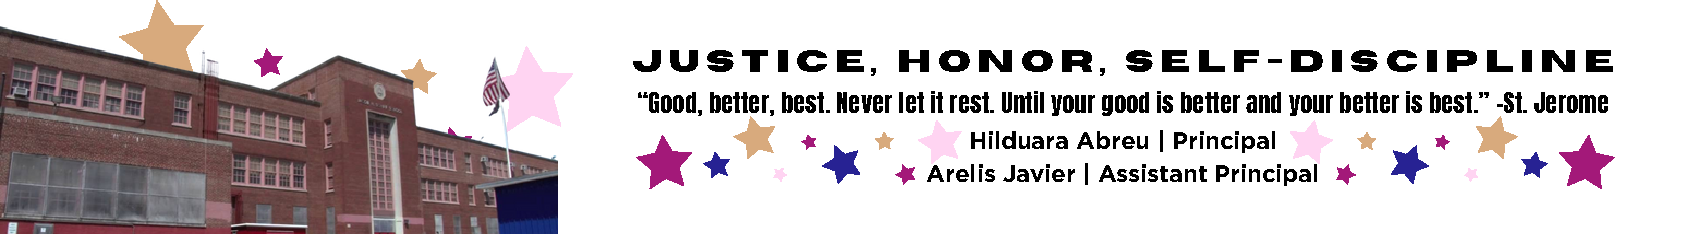
\includegraphics[width=8.8in,height=1.3in]{logo-1}}\end{picture}}
\fancyhead[C]{\setlength{\unitlength}{1in}\begin{picture}(5,0)\put(-1.9,-1){
\includegraphics[width=8.9in,height=1.3in]{logo-2}}\end{picture}}
\pagenumbering{gobble}
\usepackage{tcolorbox}
\newtcolorbox{redbox}[1][]{
  colback=red!5!white,
  colframe=red!75!black,
  fonttitle=\bfseries,
  coltitle=black,
  enhanced,
  attach boxed title to top center={yshift=-2mm},
  title=#1,
  boxed title style={colback=red!50!white}
}
\vspace*{0.3in}

Subject: Carta de Bienvenida | Año Escolar: \href{https://www.ps192.org}{2024-25}

Queridas familias de P.S. 192, grados K-5,

A medida que nos acercamos al inicio del nuevo año escolar 2024-25, que comenzará el 5 de septiembre, les extendemos una cálida bienvenida a todos nuestros estudiantes. Confiamos en que hayan tenido un agradable y saludable receso de verano. Nuestro dedicado y compasivo equipo de educadores y personal escolar anticipa con entusiasmo su regreso para lo que promete ser un año lleno de emoción, risas y aprendizaje.

Mientras nos preparamos para el regreso de su hijo/a, queremos compartir información importante que está vigente en PS 192 para garantizar una experiencia de aprendizaje segura y agradable para todos. Por favor, tomen nota de las siguientes pautas:

\begin{redbox}[Pautas a seguir]
\begin{itemize}
    \item \textbf{Llegada:} Este año, TODOS los estudiantes de grados K-5 ingresarán a través de la Cafetería cada mañana, a partir de las 7:40 AM, para desayunar.
    \item \textbf{Salida:} Este año, TODOS los estudiantes de grados K-5 serán despedidos desde el patio a las 2:15 PM. Habrá lugares designados para cada clase por grado. Por favor, sigan las señales.
\end{itemize}
\end{redbox}

Material escolar: PS 192 proporcionará todos los materiales escolares básicos, como cuadernos, carpetas y crayones. Solo pedimos que las familias de grados K-5 provean a los estudiantes con una mochila y una caja de bolsas Ziplock de tamaño galón para que los estudiantes las utilicen en los centros, en las bolsas de libros y en los kits de herramientas matemáticas.

Es un honor ser parte de una comunidad donde padres, maestros, personal y estudiantes trabajan juntos para fomentar relaciones sólidas que promueven el crecimiento académico y social. Anticipamos con entusiasmo su participación en los eventos programados a lo largo del año escolar y valoramos su compromiso activo en la educación de su hijo/a.

Las actualizaciones regulares sobre eventos en toda la escuela se comunicarán a través de nuestro sitio web: \href{https://www.ps192.org}{www.ps192.org}, \href{https://www.classdojo.com/}{ClassDojo}, School Messenger y nuestro grupo de WhatsApp. Si tienen alguna pregunta, no duden en ponerse en contacto con nuestra Coordinadora de Padres, Angela Rijo, en \href{mailto:arijo@schools.nyc.gov}{arijo@schools.nyc.gov}, sitio web de la escuela: \href{https://www.ps192.org/angela}{www.ps192.org/angela}, o al (212) 775-9560.

Estaremos organizando eventos durante todo el año y esperamos asociarnos con ustedes tanto en persona como de forma virtual. Estén atentos para obtener más información sobre todos nuestros próximos eventos:

\pagebreak
\vspace*{2cm}

RESERVEN LA FECHA:

\begin{itemize}
    \item El 12 de septiembre, organizaremos nuestro primer Encuentro Virtual con el Maestro de su hijo de 4:30 PM a 7:30 PM
\end{itemize}

Estamos contando los días con entusiasmo hasta poder darles la bienvenida de nuevo el jueves, 5 de septiembre de 2024. Es un honor servir como directora de PS 192 y extiendo mi más sincero agradecimiento por su cooperación y dedicación al bienestar de nuestros niños, personal y escuela.

En unidad,


\includegraphics[width=0.2\textwidth]{hil_signature}

\textbf{Principal}

\textit{La Escuela donde El Aprendizaje es Divertido!}

\href{https://www.ps192.org}{www.ps192.org}
\end{document}
